\documentclass[a4paper,12pt,oneside]{book}
\usepackage[export]{adjustbox}
\usepackage{graphicx}
\usepackage[margin=2cm]{geometry}
\usepackage{color}
\usepackage{fix-cm}  
\usepackage{fancyhdr}  


\usepackage[scale=2,opacity=0.1,angle=0]{background}
\backgroundsetup{contents={
\includegraphics{logo}}}

\definecolor{Dred}{RGB}{210,0,0}
\definecolor{Dblue}{RGB}{0,0,150}


\begin{document}
%\maketitle
%\tableofcontents
\begin{titlepage}
\hspace{5cm}
\textit{\textcolor{Dblue}{\textbf{\fontsize{60}{70}\selectfont{Fi-Pi}}}}
\\\\\\\\\\
\textcolor{Dred}{\textbf{\fontsize{30}{10}\selectfont{Adaptor Board for Firebird V Robot}}}
\\\\\
\textcolor{Dred}{\textbf{\fontsize{30}{10}\selectfont{\hspace{4 cm}using Raspberry Pi 2}}}
\\\\\\\\
\textcolor{Dred}{\textbf{\fontsize{30}{10}\selectfont{\hspace{3 cm}HARDWARE MANUAL}}}
\\\\\\\\

\begin{figure}[h]
		\hspace{2cm}
	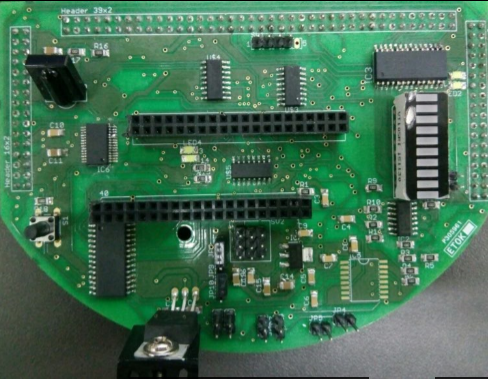
\includegraphics[width=0.8\textwidth]{pcb}
\end{figure}
\hfill
\end{titlepage}
\pagebreak

\pagestyle{fancy}
\fancyhf{}
\rhead{Fi-Pi hardware manual}
\lfoot{www.e-yantra.org}
\rfoot{Page \thepage}
.\\
\textbf{\fontsize{10}{10}\selectfont{Documentation author}}
\\\\
\hspace{5cm}
Milan Preet Singh
\\\
Tejaswini A
\\\\
\textbf{\fontsize{10}{10}\selectfont{Mentors}}
\\\\
\hspace{5cm}
Rutuja Ekatpure
\\\
Deepa Avudiappan
\pagebreak

\pagestyle{fancy}
\fancyhf{}
\rhead{Fi-Pi hardware manual}
\lfoot{www.e-yantra.org}
\rfoot{Page \thepage}
\tableofcontents{}
\pagebreak
\chapter{}
\section{\textbf{Introduction}}

Currently Firebird V robot comes with ATMEGA2560, 8051, ARM7 adaptor board. Using a raspberry pi based adaptor board would add to the functionality of the robot. The idea is to integrate the features of Rpi to Firebird V robot.This would facilitate any on-board computations, image processing(Rpi supports PiCamera directly), the robot could even be used for IOT (Internet Of Things) applications. Because of the presence of an operating system, Rpi is a mini computer.Adaptor board for Firebird V would definitely be an advantage.\\
\hfill

\subsection{\textbf{Components on the adaptor board}}
\vspace{1cm}
\begin{itemize}
	\item{MCP3008 (8 channel 10-bit ADC)}
	\item{MCP23017 Port expander IC}
	\item{Header pins for interfacing adaptor board with main board, raspberry pi and for the expansion socket.}
	\item{FT232 for USB communication}	
	\item{MAX202 for RS232 communication}
	\item{LM324 quad comparator IC}
	\item{Bar Graph LED}
	\item{L7805 IC for powering Rpi}
	\item{LM1117 IC for powering servo motors}
	\item{Switches}
    \item{Jumpers}
    \item{Resistors,capacitors,diodes,LEDs}	
\end{itemize}
\pagebreak

\section{\textbf{Main board pin details}}
\begin{figure}[h]
	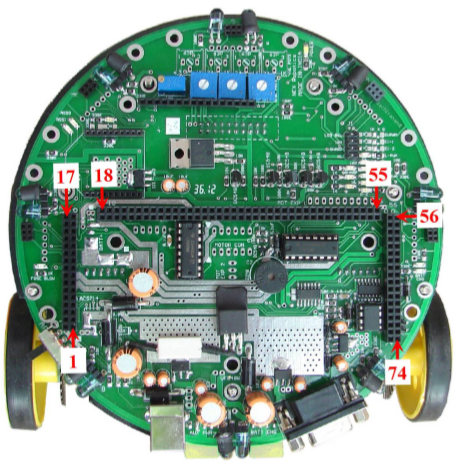
\includegraphics[width=1.\textwidth]{main_board}
	\caption{Firebird V - Main Board}
\end{figure}
\hspace{7cm}Table 2.\\
\begin{tabular}{|p{2cm}|p{3cm}|p{6cm}|p{5cm}|}
	
	\hline
\textbf{Main board Pin No.} & \textbf{Pin Name} & \textbf{Function} & connections on adaptor board\\ [0.5ex] 
\hline
1. & CS\* &Current sense analog value &  \\ 
\hline
2. & IR Proximity sensor 8 &IR Proximity sensor 8 analog value & ADC1, Channel7 \\ 
\hline
3. &Ground &Ground & ground \\ 
\hline
\end{tabular}

\begin{tabular}{|p{2cm}|p{3cm}|p{6cm}|p{5cm}|}
	\hline
4. &USB Data+ &USB connection going to the raspberry pi via FT232 USB to serial converter.To enable USB communication set jumper as shown.& Connected to USBDP of FT232.  \\ 
\hline

5. &USB Data- &USB connection going to the raspberry pi via FT232 USB to serial converter.To enable USB communication set jumper as shown.& connected to USBDM of FT232. \\ 
\hline

6. &VUSB &Voltage source for FT232& Used for powering FT232. \\ 
\hline
	7. &5V System &5V System Voltage. Can be used for powering up any digital device with current limit of 400mA. & Used in Battery voltage sensing circuit.  \\ 
	\hline
8. &5V Sensor &5V Sensor Voltage. Can be used for additional sensor interfacing with current limit 300mA. &  \\ 
\hline
9. &5V Sensor &5V Sensor Voltage. Can be used for additional sensor interfacing with current limit 300mA.& \\ 
\hline
	10. &5V System &5V System Voltage. Can be used for powering up any digital device with current limit of 400mA. & Used in Battery voltage sensing circuit.  \\ 
\hline
	11. &Sharp IR Range Sensor 1 &Analog output of Sharp IR range Sensor 1& ADC2, Channel 0 \\ 
	\hline
12. &IR Proximity Sensor 1 &Analog output of IR Proximity Sensor 1.& ADC1, Channel 0. \\ 
\hline
	13. &XBee RXD & XBee wireless module serial data in &connected to raspberry pi TX via jumper 2. \\ 
	\hline
14. &XBee TXD & XBee wireless module serial data out &connected to raspberry pi RX via jumper 3.  \\ 
\hline
15. &Sharp IR Range Sensor 2 &Analog output of Sharp IR range Sensor 2& ADC2, Channel 1 \\ 
\hline
16. &IR Proximity Sensor 2 &Analog output of IR Proximity Sensor 2& ADC1, Channel 1. \\ 
\hline
17A. &RSSI &To capture the RSSI signal& \\
\hline
17B.& Ultrasonic Trigger& To give trigger for Ultrasonic sensor& \\
\hline
18.& MOSI & not used & \\
\hline
19.& MISO & not used & \\
\hline
20.& SCK & not used & \\
\hline 
21.& SSI & not used & \\
\hline
22. & RS & LCD Register select pin(Command) &connected to GPIO 21 of raspberry pi\\
\hline
23. & RW & LCD Write pin(Command) & Ground\\
\hline
24. & EN & LCD Enable pin(Command) & connected to GPIO 26 of raspberry pi\\
\hline
\end{tabular}

\begin{tabular}{|p{2cm}|p{3cm}|p{6cm}|p{5cm}|}
	\hline
25. & DB5 & LCD Data bit 5& connected to GPIO 19 of raspberry pi\\
\hline
26. & DB4 & LCD Data bit 4& connected to GPIO 13 of raspberry pi\\
\hline
27. & DB5 & LCD Data bit 6&connected to GPIO 6 of raspberry pi\\
\hline
28. & DB5 & LCD Data bit 7& connected to GPIO 5 of raspberry pi\\
\hline
29. & V Battery System & 9-12V unregulated power supply for additional module interfacing. & connected to input pin of L7805 for powering Rpi. \\
\hline
30. & White Line sensor 1 & Analog output of White Line sensor 1 &ADC2, Channel 5\\
\hline
31. & White Line sensor 2 & Analog output of White Line sensor 2 &ADC2, Channel 6\\
\hline

32. & White Line sensor 3 & Analog output of White Line sensor 3& ADC2,Channel 7 \\
\hline
33. & Sharp IR Sensor 1 to 5 Disable &TTL or CMOS input.Disable IR range Sensor & GPB5, port expander 1.\\
\hline
34. &IR Proximity Sensor Disable &TTL or CMOS input.Disable IR range Sensor &  GPB6, port expander 1\\
	\hline
35. &5V System &5V System Voltage. Can be used for powering up any digital device with current limit of 400mA&  \\ 
\hline
36. & White Line sensor 4 & Analog output of White Line sensor 4 &Can be connected externally to port expansion socket via jumpers.\\
\hline
37. & White Line sensor 5 & Analog output of White Line sensor 5&Can be connected externally to port expansion socket via jumpers.\\
\hline
38. & White Line sensor 6 & Analog output of White Line sensor 6&Can be connected externally to port expansion socket via jumpers.\\
\hline
39. & White Line sensor 7 & Analog output of White Line sensor 7&Can be connected externally to port expansion socket via jumpers.\\
	\hline
40. & White Line Sensor Disable &TTL or CMOS input.Disable White Line Sensor& GPB7, port expander 1\\
\hline
41. &Sharp IR Range Sensor 3 &Analog output of Sharp IR range Sensor 3&ADC2, Channel2  \\ 
\hline
42. &IR Proximity Sensor 3 &Analog output of IR Proximity Sensor 3.&ADC1, Channel 2 \\ 
\hline
43. &IR Proximity Sensor 4 &Analog output of IR Proximity Sensor 4.& ADC1, Channel 3 \\
\hline 
44. &Sharp IR Range Sensor 4 &Analog output of Sharp IR range Sensor 4& ADC2, Channel 3 \\
\hline 
45. &Sharp IR Range Sensor 5 &Analog output of Sharp IR range Sensor 5& ADC2, Channel 4  \\ 
\hline
\end{tabular}

\begin{tabular}{|p{2cm}|p{3cm}|p{6cm}|p{5cm}|}
	\hline
46. &IR Proximity Sensor 5 &Analog output of IR Proximity Sensor 5.& ADC1, Channel 4  \\
\hline
47. & C1 1 & Logic input 1 for C1 Motor Drive& not connected\\
\hline
48. & C1 PWM & PWM input for C1 Motor Drive& not connected\\
\hline
49. & C1 2 & Logic input 2 for C1 Motor Drive& not connected\\
\hline
50. & PWML & PWM input for Left Motor Drive&GPA5, port expander 1\\
\hline
51. & L1 & Logic input 1 for Left Motor Drive& GPA4, port expander 1\\
\hline
52. & L2 & Logic input 2 for Left Motor Drive &GPA3, port expander 1\\
\hline
53. & R1 & Logic input 1 for Right Motor Drive&GPA2, port expander 1\\
\hline
54. & PWMR & PWM input for Right Motor Drive&GPA1, port expander 1\\
\hline
55. & R2 & Logic input 2 for Right Motor Drive&GPA1, port expander 1\\
\hline
56. & & Not Used&\\
\hline
57. & & Not Used&\\
\hline
58. & & Not Used&\\
\hline
59. & & Not Used&\\
\hline
61. & & Not Used&\\
\hline
62. &Position Encoder Left &Output of Left Position Encoder (0-5V)&raspberry pi GPIO 17\\
\hline
63. &Position Encoder Right &Output of Right Position Encoder (0-5V)&raspberry pi GPIO 27\\
\hline
64. &Position Encoder C2 &Output of C2 Position Encoder (0-5V)&not used\\
\hline
65. &Position Encoder C1 &Output of C1 Position Encoder (0-5V)&not used\\
\hline
66. & C2 2 & Logic input 2 for C2 Motor Drive&not used\\
\hline
67. & C2 1 & Logic input 1 for C2 Motor Drive&not used\\
\hline
68. & C2 PWM & PWM input for C2 Motor Drive&not used\\
\hline
69. &IR Proximity Sensor 6 &Analog output of IR Proximity Sensor 6.&ADC1, Channel 5 \\
\hline
70. &IR Proximity Sensor 7 &Analog output of IR Proximity Sensor 7.&ADC1, Channel 6 \\
\hline
71. &Buzzer &Input, V>0.65V turns on the buzzer &raspberry pi GPIO 4\\
\hline
72. &DAC OUT &Not Connected& \\
\hline
73. &RS232 TXD & RS232 Transmit, connected to DB9 serial connector on main board & Connected to MAX202 \\
\hline


 
\end{tabular}
\pagebreak 
\section{\textbf{Adaptor board parts}}
\begin{figure}[h]
	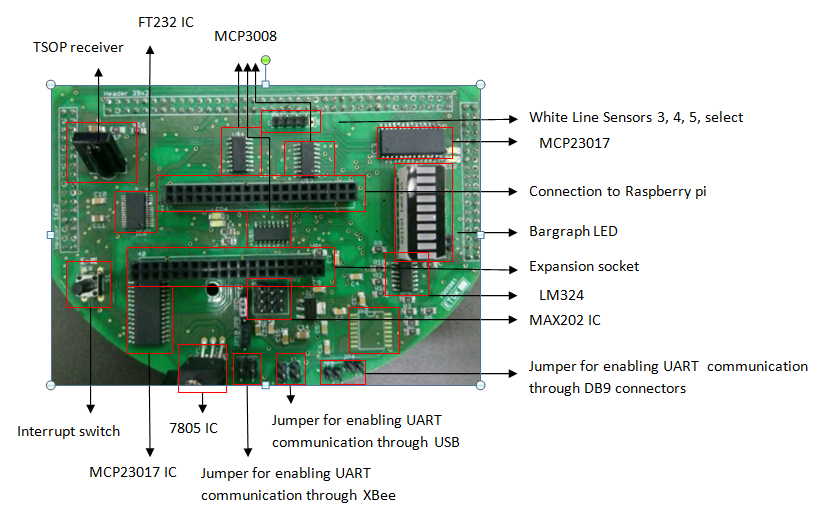
\includegraphics[width=1.1\textwidth]{Adaptor_board}
	\caption{Adaptor board}
\end{figure}
\pagebreak

\section{\textbf{Powering Raspberry Pi}}
\begin{figure}[h]

	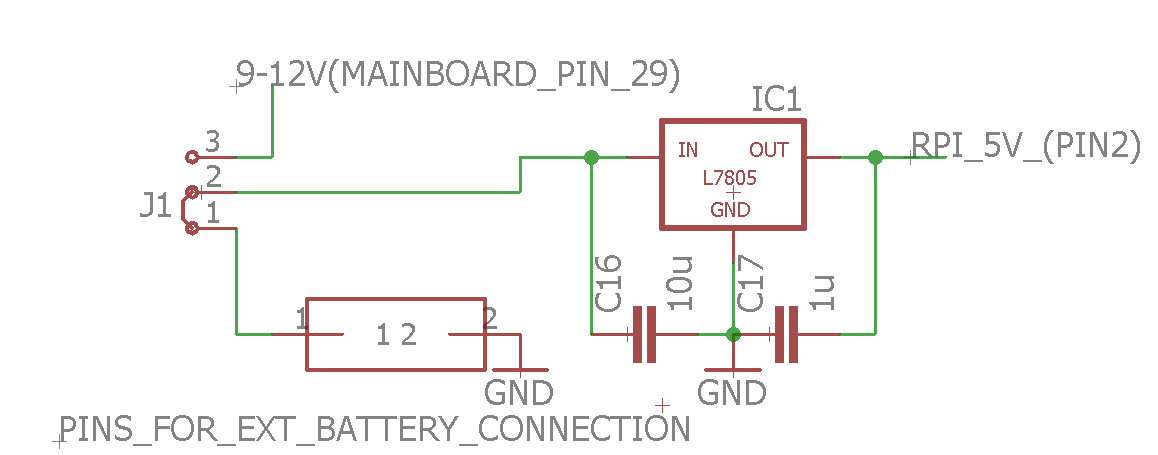
\includegraphics[width=1.\textwidth]{rpi_power}
	\caption{Powering raspberry pi}
\end{figure}
\hfill
\begin{itemize}
	\item{Raspberry pi needs a constant 5v and more than 1A power supply. L7805 voltage regulator is used to serve this purpose.}
	\item {The battery voltage of Firebird V robot is directly obtained by using pin 29 of main board.}
	\item {The output of 29th pin on the main board is in the range of 9-12v. Either this or any external battery can be used as an input for the 7805 IC. The selection between the two is facilitated by a jumper.}
	\item {The output of 7805 is the regulated 5v output, which is given to 5v pin of raspberry pi.}
	\item {Two header pins are provided for the connection with external battery.}
\end{itemize}
\pagebreak

\section{\textbf{Battery voltage indication}}

\begin{figure}[h]
	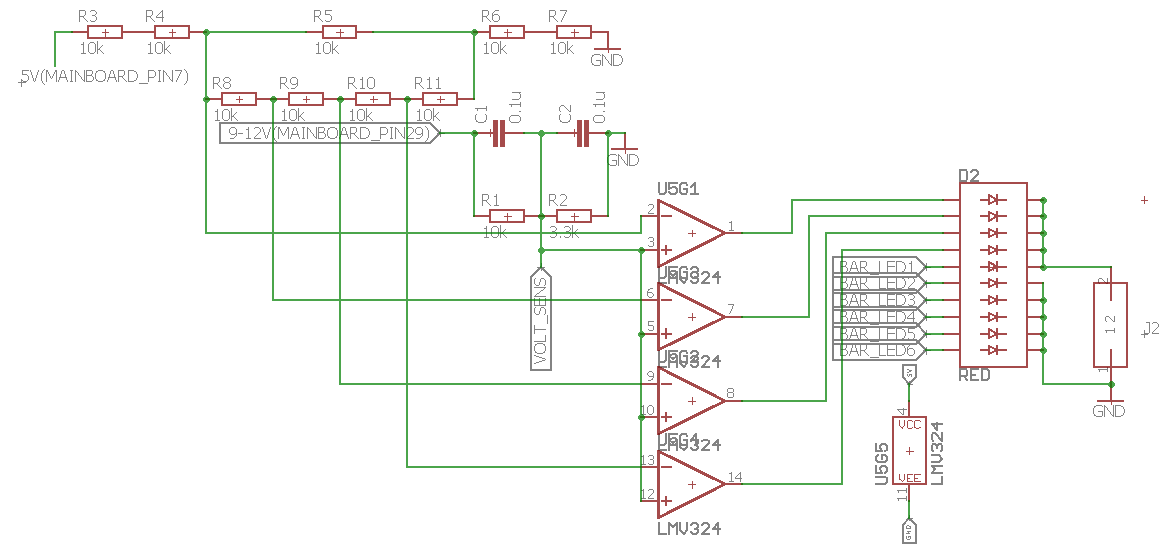
\includegraphics[width=1\textwidth]{volt_sens}
		\caption{voltage sensing circuit}
\end{figure}
\hfill
\begin{itemize}
	\item{The battery voltage of the Firebird V robot can be detected by the battery voltage sensing circuit.}
	\item{It could be sensed either by connecting the volt\_sens pin to ADC and reading its value or by seeing the indications from the bottom 5 LEDs of bargraph LEDs}
	\item{First of all, the 9-12v output from mainboard pin 29 is mapped to value less than 5V by using the voltage divider circuit.This circuit apprx divides the voltage by 4 and henceforth mapping 12V to 3V, 11V to 2.75V, 10V to 2.5V and 9V to 2.25V.This output is given to all 4 input+ pins of the quad comparator IC LM324.}
	\item{The input for input- pins are given as 3V, 2.75V, 2.5V, 2.25V resp by the simple circuit as given above.}
	\item{So, whenever voltage is greater than 12V all the bottom 5 LEDs glow, when greater than 11V and less than 12V bottom 4 LEDs glow, when greater than 10V and less than 11V bottom 3 LEDs glow and when greater than 9V and less than 10V bottom 2 LEDs glow.}
	\item {In order to see the battery status, jumper J8 has to be inserted into the two header pins provided at the right of the bargraph LED.}
\end{itemize}
\pagebreak

\section{\textbf{Buzzer interface}}
\begin{figure}[h]
	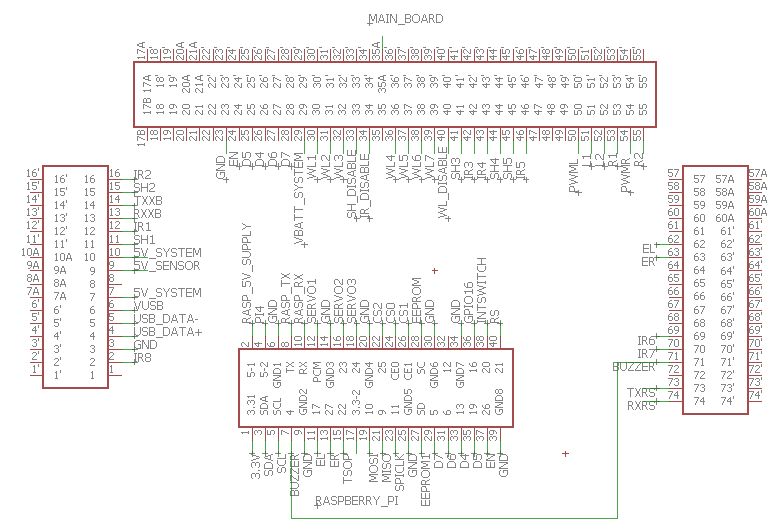
\includegraphics[width=1\textwidth]{buzzer}
	\caption{Buzzer interface}
\end{figure}
\hfill
\begin{itemize}
	\item {Input for buzzer is available at pin 71 of main board.}
	\item {This input is given to GPIO pin 4 of raspberry pi.}
	\item {In order to program it, this pin should be used.}
\end{itemize}
\pagebreak

\section{\textbf{LCD interface}}
\begin{figure}[h]
	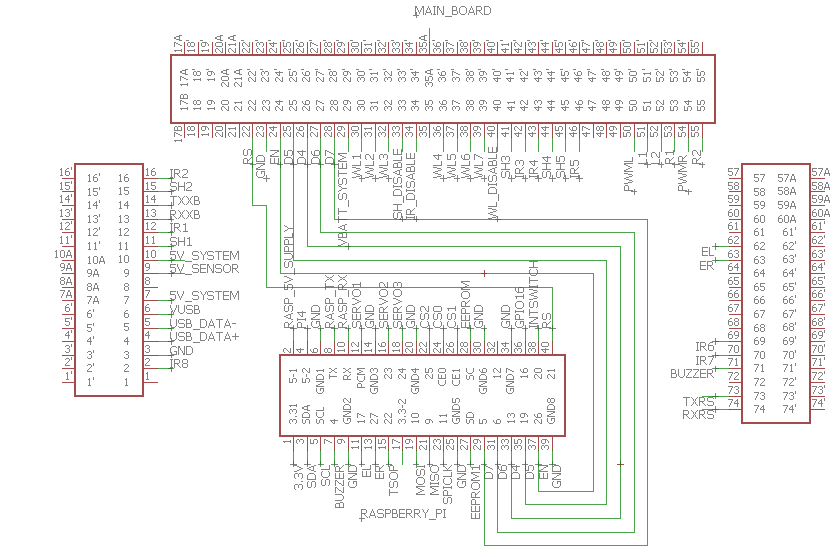
\includegraphics[width=1\textwidth]{lcd}
	\caption{LCD interface}
\end{figure}
\hfill
\begin{itemize}
	\item {LCD pins RS, EN, DB5, DB4, DB6 and DB7 are available on pins 22, 24, 25, 26, 27 and 28 resp. on the mainboard.}
	\item {These are give to pins 21, 26, 19, 13, 6 and 5 GPIO pins of raspberry pi resp.}
	\item {The RW pin of LCD is grounded.}
	\item {In order to program the LCD, these pins should be used.}
\end{itemize}
\pagebreak

\section{\textbf{Sensors and ADC interface}}
\begin{figure}[h]
	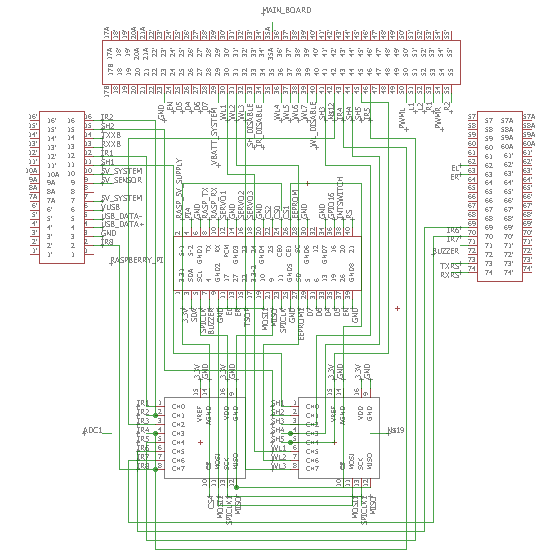
\includegraphics[width=1\textwidth]{adc}
	\caption{Sensors and ADC interface}
\end{figure}
\hfill
\begin{itemize}
	\item {Sensors values are read by raspberry pi via external ADC. Raspberry pi communicates to ADC MCP3008 with SPI communication protocol.}
	\item {The communication between raspberry pi and MCP3008 happens with 3 lines, which are MISO, MOSI and SCLK.These pins are common to all 3 ADCs. The appropriate device is chosen by its chip select pin which is unique for every device.}
	\item {The chip select pin of ADC1 and ADC2 are given to CE0 and CE1 pins of raspberry pi resp.}
	\item {There are 3 MCP3008 ADCs on adaptor board. Any external sensor can be connected to ADC3, the pins of which are available on the adaptor board expansion socket.The chip select CS2 for this ADC is given by GPIO 15 of raspberry pi.}
	\item {All the 8 IR proximity sensors are connected to ADC1, White line sensors and sharp IR sensors are given to ADC2.}\\
\end{itemize}
\hspace{7cm}Table 2.\\\\
\begin{tabular}{|p{2cm}|p{5cm}|p{2cm}|p{5cm}|}
	\hline
	\textbf{No.} &\textbf{Sensor} & \textbf{ADC Name} & \textbf{Channel No.}\\ [0.5ex] 
	\hline
	1. & IR Proximity sensor 1 & ADC1 & Channel 0  \\ 
	\hline
	2. & IR Proximity sensor 2 & ADC1 & Channel 1  \\ 
	\hline
	3. & IR Proximity sensor 3 & ADC1 & Channel 2 \\ 
	\hline
	4. & IR Proximity sensor 4 & ADC1 & Channel 3 \\ 
   \hline
	5. & IR Proximity sensor 5 & ADC1 & Channel 4  \\ 
   \hline
	6. & IR Proximity sensor 6 & ADC1 & Channel 5  \\ 
  \hline
	7. & IR Proximity sensor 7 & ADC1 & Channel 6  \\ 
  \hline
  	8. & IR Proximity sensor 8 & ADC1 & Channel 7  \\ 
  \hline
  	9. & Sharp IR sensor 1 & ADC2 & Channel 0  \\ 
  \hline
  	10. & Sharp IR sensor 2 & ADC2 & Channel 1  \\ 
  \hline
  	11. & Sharp IR sensor 3 & ADC2 & Channel 2  \\ 
  \hline
  	12. & Sharp IR sensor 4 & ADC2 & Channel 3  \\ 
  \hline
  	13. & Sharp IR sensor 5 & ADC2 & Channel 4  \\ 
  \hline
  	14. & White Line sensor 1 & ADC2 & Channel 5  \\ 
  \hline
	15. & White Line sensor 2 & ADC2 & Channel 6  \\ 
\hline
	16. & White Line sensor 3 & ADC2 & Channel 7  \\ 
\hline
	
\end{tabular}
\pagebreak

\section{\textbf{Motors and wheel encoders interface}}
\begin{figure}[h]
	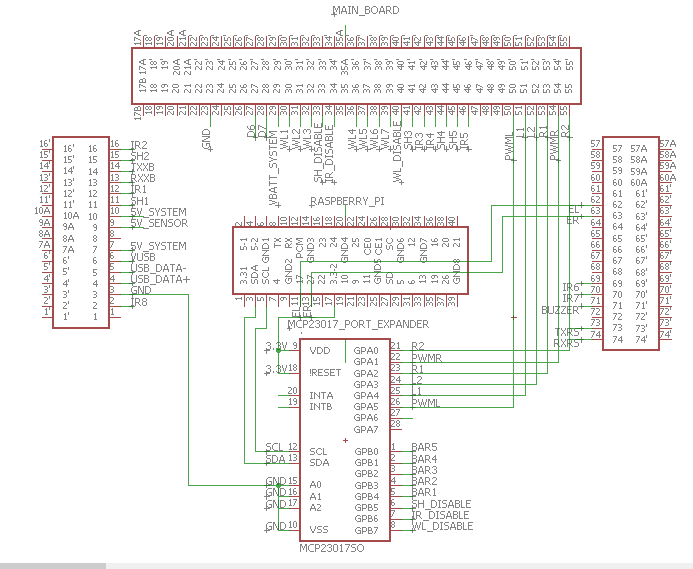
\includegraphics[width=1\textwidth]{wheels}
	\caption{Motors and wheel encoders interface}
\end{figure}
\hfill
\begin{itemize}
	\item {Left motor control pins(L1,L2), Right motor control pins(R1,R2)and PWM motor control pins(PWMl, PWMR) are available on pins 51, 52, 53, 55, 50 and 54 pins of main board resp.}
	\item {The above mentioned pins are connected to MCP23017 Port expander 1 with I2C communication.This would facilitate the usage of more GPIO pins since raspberry pi doesn't have many(27 GPIOs available).}
	\item {The GPIO pins of port expander 2 is given to the adaptor board expansion socket.}
	\item {Data and clk signals flow through SDA and SCL lines resp between Raspberry pi and MCP23017 port expander.These lines are common for both the port expanders.}
	\item {The address of this Port expander as shown in fig.7 is 20 (000) and that of 2nd is 21 (001) which is specified by voltage levels at A0, A1, A2 pins resp.}
	\item {R2, PWMR, R1, L2, L1 and PWML pins are available on GPA0, GPA1, GPA2, GPA3, GPA4, GPA5 and GPA6 resp. of the Port expander.}
   	\item {The Left and Right wheel encoders are connected to the GPIO 17 and 27 pins of raspberry pi.}
\end{itemize}
\pagebreak

\section{\textbf{Powering servo motors and Servo pod connections}}
\begin{figure}[h]
	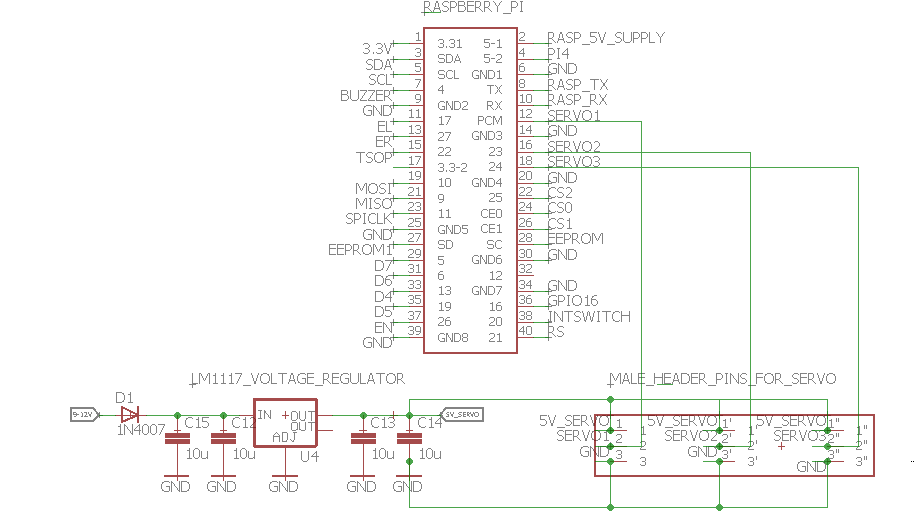
\includegraphics[width=1\textwidth]{servo}
	\caption{Powering servo motors and Servo pod connections}
\end{figure}
\hfill
\begin{itemize}
	\item {Servo motors need 5V and more than 500mA current to run efficiently. In order to meet these requirements, the +ve of servo motors is given to the output of LM1117 Voltage regulator IC. The input to which is given by 9-12V (pin 29) from main board.}
	\item {A set of 9 male header pins are given on the Adaptor board for interfacing upto 3 servo motors.}
	\item {Three of which are for Vcc (5V), three for ground and three for controlling th motion of servo motors 1,2 and 3 resp.}
	\item {The servo motor control pins are given to GPIO 5, 23 and 24 pins of raspberry pi resp. }
\end{itemize}
\pagebreak

\section{\textbf{Interrupt switch and controlling bargraph leds}}
\begin{figure}[h]
	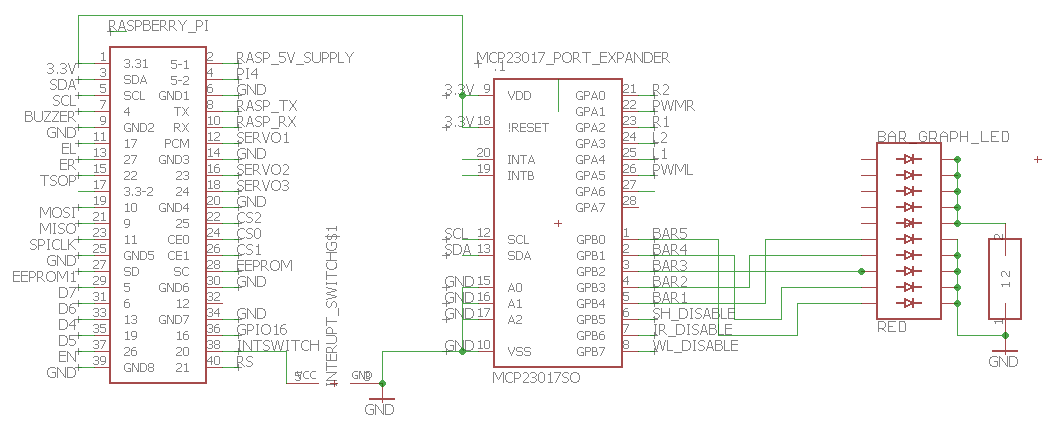
\includegraphics[width=1\textwidth]{interupt_bargraph}
	\caption{Interrupt switch and controlling bargraph leds}
\end{figure}
\hfill
\begin{itemize}
	\item {Sudden power cut to raspberry pi may lead to spoiling of the Raspbian OS. Hence, whenever the interrupt switch is pressed on the adaptor board, a python script could be written such that the raspberry pi shuts down systematically.}
	\item {The bottom 5 LEDs of bargraph LED can be controlled by the GPB0,  GPB1, GPB2, GPB3 and GPB4 pins of MCP23017 port Expander.}
\end{itemize}
\pagebreak

\section{\textbf{TSOP1738 RC5 IR receiver and decoder}}
\begin{figure}[h]
	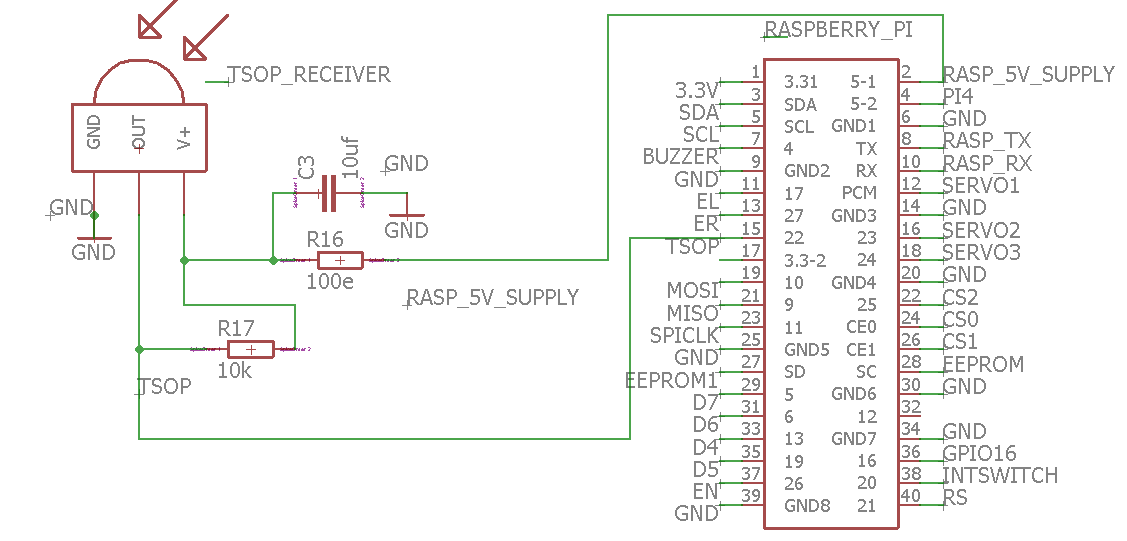
\includegraphics[width=1\textwidth]{tsop}
	\caption{TSOP1738 RC5 IR receiver and decoder}
\end{figure}
\hfill
\begin{itemize}
	\item {The Firebird V robot can run according to the commands of TV remote, by decoding the IR signals which it receives from the TSOP receiver. }
	\item {It has Vcc(3.3V), ground and the output pin, which is connected to GPIO 22 pin rsapberry pi.}
	\item {By decoding the data obtained from the IR signals of TV remote, the robot could run accordingly.}
\end{itemize}
\pagebreak

\section{\textbf{UART communication with Raspberry Pi}}
\begin{figure}[h]
	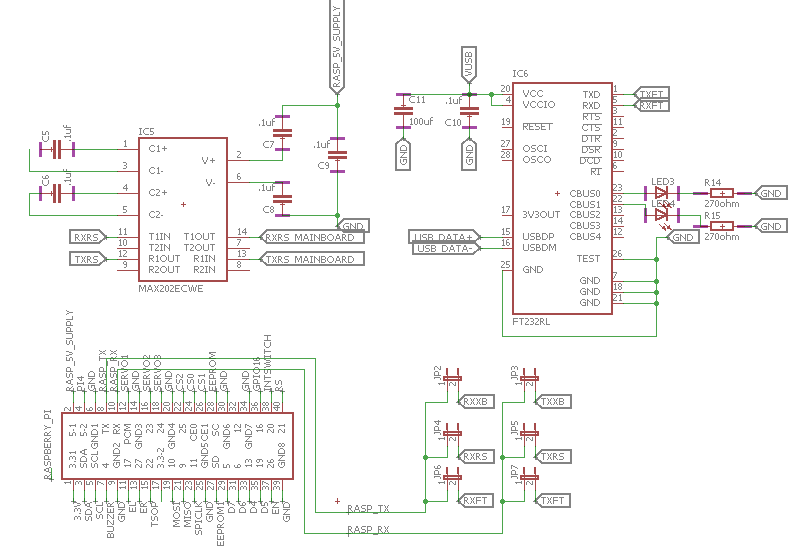
\includegraphics[width=1\textwidth]{UART}
	\caption{UART communication with Raspberry Pi}
\end{figure}
\hfill
\begin{itemize}
	\item {Raspberry Pi has only 1 set RX-TX pins for UART communication.}
	\item {But, Firebird V robot has 3 modes of serial communication which are through DB9 connectors, USB cable and through XBee.}
	\item {In order to use these 3 modes, 3 pairs of jumpers J2-J3, J4-J5 and J6-J7 are provided for completing the TX-RX circuit of XBee, DB connector and USB cable with the TX and RX pins of raspberry pi resp.}
	\item { FT232 USB to serial converter is used for UART communication via USB cable.}
	\item { TTL to RS232 converter is used for the UART serial communication with DB9 connectors.}
	\item {USB+ and USB- pins are available on pins 4 and 5 of main board resp.}
    \item {RS232 TXD and RXD are available on pins 73 and 74 of main board resp.}
     \item {XBee TXD and RXD are available on pins 14 and 13 of main board resp.}
	
\end{itemize}
\pagebreak

\section{\textbf{Adaptor board expansion socket}}
\begin{figure}[h]
	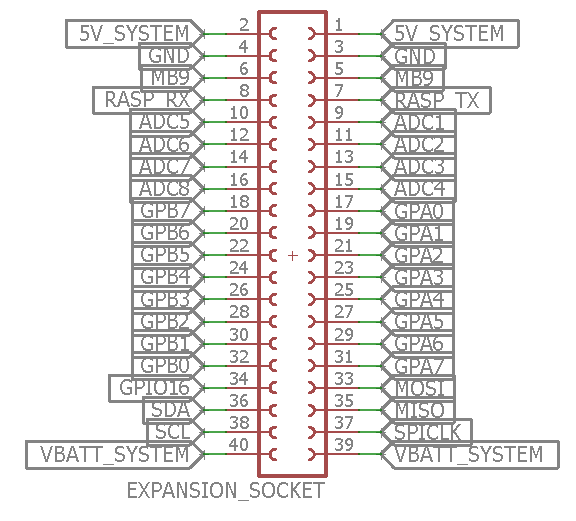
\includegraphics[width=1\textwidth]{expansion}
	\caption{Adaptor board expansion socket}
\end{figure}
\begin{itemize}
	\item {If the attachment of other external sensors or any other device to the Firebird V robot is required, they could be connected to the Adaptor board expansion slot.}
	\item {The expansion slot has ADC channel pins, GPIOs connected to port expander, ground, 5V, 9V pins, TX-RX, SPI lines(MISO, MOSI, SPICLK) and I2C lines(SDA,SCL). }
	\item {With the help of these pins present on expansion socket, any device could be connected to the robot. }
\end{itemize}

\pagebreak
\hspace{3cm}Table 3.\\\\
\begin{tabular}{|p{2cm}|p{10cm}|}
	\hline
	\textbf{Pin No.} & \textbf{Connected to} \\ [0.5ex]
	\hline 
	1. & 5V System\\
	\hline
		2. & 5V System\\
	\hline
		3. & Ground\\
	\hline  
        4. & Ground\\
    \hline	
    	5. &Main board pin 9\\
	\hline
		6. & Main board pin 9\\
	\hline
		7. & Raspberry pi TX\\
	\hline
		8. &  Raspberry pi RX\\
	\hline
	9. &ADC3 Channel 0 (chipselect on Rpi GPIO 15)\\
\hline
	10. &ADC3 Channel 1 (chipselect on Rpi GPIO 15)\\
\hline
	11. &ADC3 Channel 2 (chipselect on Rpi GPIO 15)\\
\hline
	12. &ADC3 Channel 3 (chipselect on Rpi GPIO 15)\\
\hline
	13. &ADC3 Channel 4 (chipselect on Rpi GPIO 15)\\
\hline
	14. &ADC3 Channel 5 (chipselect on Rpi GPIO 15)\\
\hline
	15. &ADC3 Channel 6 (chipselect on Rpi GPIO 15)\\
\hline
    16. &ADC3 Channel 7 (chipselect on Rpi GPIO 15)\\
\hline
 17. &Port Expander 2, GPA0 (Device address 22)\\
\hline
 18. &Port Expander 2, GPB7 (Device address 22)\\
\hline
 19. &Port Expander 2, GPA1 (Device address 22)\\
\hline
 20. &Port Expander 2, GPB6 (Device address 22)\\
\hline
 21. &Port Expander 2, GPA2 (Device address 22)\\
\hline
 22. &Port Expander 2, GPB5 (Device address 22)\\
\hline
 23. &Port Expander 2, GPA3 (Device address 22)\\
\hline
 24. &Port Expander 2, GPB4 (Device address 22)\\
\hline
 25. &Port Expander 2, GPA4 (Device address 22)\\
\hline
 26. &Port Expander 2, GPB3 (Device address 22)\\
\hline
 27. &Port Expander 2, GPA5 (Device address 22)\\
\hline
 28. &Port Expander 2, GPB2 (Device address 22)\\
\hline
 29. &Port Expander 2, GPA6 (Device address 22)\\
\hline
 30. &Port Expander 2, GPB1 (Device address 22)\\
\hline
 31. &Port Expander 2, GPA7 (Device address 22)\\
\hline
 32. &Port Expander 2, GPB0 (Device address 22)\\
\hline
33. & Rpi MOSI\\
\hline
34. & Rpi GPIO 16\\
\hline
35. & Rpi MISO\\
\hline  
36. & Rpi SDA\\
\hline	
37. & Rpi SPICLK\\
\hline
38. & Rpi SCL\\
\hline
39. & VBatt system\\
\hline
40. &  VBatt system\\
\hline
	
\end{tabular}
\pagebreak 




\end{document}